%===================================================================%
\section{Public Cible \& Fonctionnalités Attendues}
%===================================================================%
Nous souhaitons créer un catalogue des APIs disponibles pour les consultants externes au SGSI ainsi que pour les développeurs internes permettant de connaître leurs intérêts pour certaines APIs.

Le produit final idéal doit présenter les capacités suivantes :
\begin{itemize}
    \item[$\rightarrow$] Présenter les APIs visuellement de manière similaire à l'interface d'API Manager (nom, icône potentielle, version, temps de la dernière mise à jour, tags potentiels) et possédant une barre de recherche ainsi que des filtres de catégorie pour faciliter la navigation du marketplace.
    \item[$\rightarrow$] Chaque API doit rediriger vers une page présentant les informations plus détaillés de l'API (swagger téléchargeable, numéro de révision, documentation, exemples de réponses, interface offrant la possibilité de demander l'accès à l'API).
    \item[$\rightarrow$] Être capable de se mettre à jour automatiquement de manière régulière ainsi que de pouvoir être mis à jour manuellement par ses administrateurs en cas de besoin.
    \item[$\rightarrow$] Offrir la possibilité de cacher certaines APIs pour certains utilisateurs selon leurs droits d'accès.
    \item[$\rightarrow$] Offrir la possibilité aux administrateurs de blacklister certaines APIs. % avant l'importation
    \item[$\rightarrow$] Permettre la suppression manuelle de certaines APIs.
\end{itemize}

%%%%%%%%%%%%%%%%%%%%%%%%%%%%%%%%%%%%%%%%%%%%%%%%%%%%%%%%%%%%%%%%%%%%%
%                                                                   %
%                                                                   %
%                                                                   %
%                                                                   %
%                                                                   %
%                                                                   %
%                                                                   %
%                                                                   %
%===================================================================%
\section{Contraintes}
%===================================================================%
\begin{itemize}
    \item[$\bullet$] Le catalogue doit rester en lecture seule pour les utilisateurs finaux qui ne peuvent pas tester les APIs.
    \item[$\bullet$] L'application doit être documentée tant au niveau de son architecture et organisation qu'au niveau du code et de son utilisation.
    \item[$\bullet$] Ce projet se fera de manière itérative semaines par semaine tout au long du stage.
\end{itemize}

%%%%%%%%%%%%%%%%%%%%%%%%%%%%%%%%%%%%%%%%%%%%%%%%%%%%%%%%%%%%%%%%%%%%%
%                                                                   %
%                                                                   %
%                                                                   %
%                                                                   %
%                                                                   %
%                                                                   %
%                                                                   %
%                                                                   %
%===================================================================%
\section{Premières Idées \& Mock-ups}
%===================================================================%
L'application doit chercher les informations concernant les APIs de manière automatique via la version en ligne de commande de l'API Manager de WSO2 : API-CTL.\\
Cette version permet de consulter les mêmes informations concernant les APIs que l'interface graphique : elle donne la possibilité de télécharger les archives .zip contenant les informations tels que les fichiers swagger, la documentation, les icônes, les produits, etc. des APIs.

\subsection{Page d'accueil}
La page d'accueil de l'application ressemblera à API Manager : une interface simple avec tuiles, icônes, barre de recherche, filtres, tags, etc. dans le même thème que la charte graphique de l'UCLouvain.

\begin{figure}[H]
    \centering
    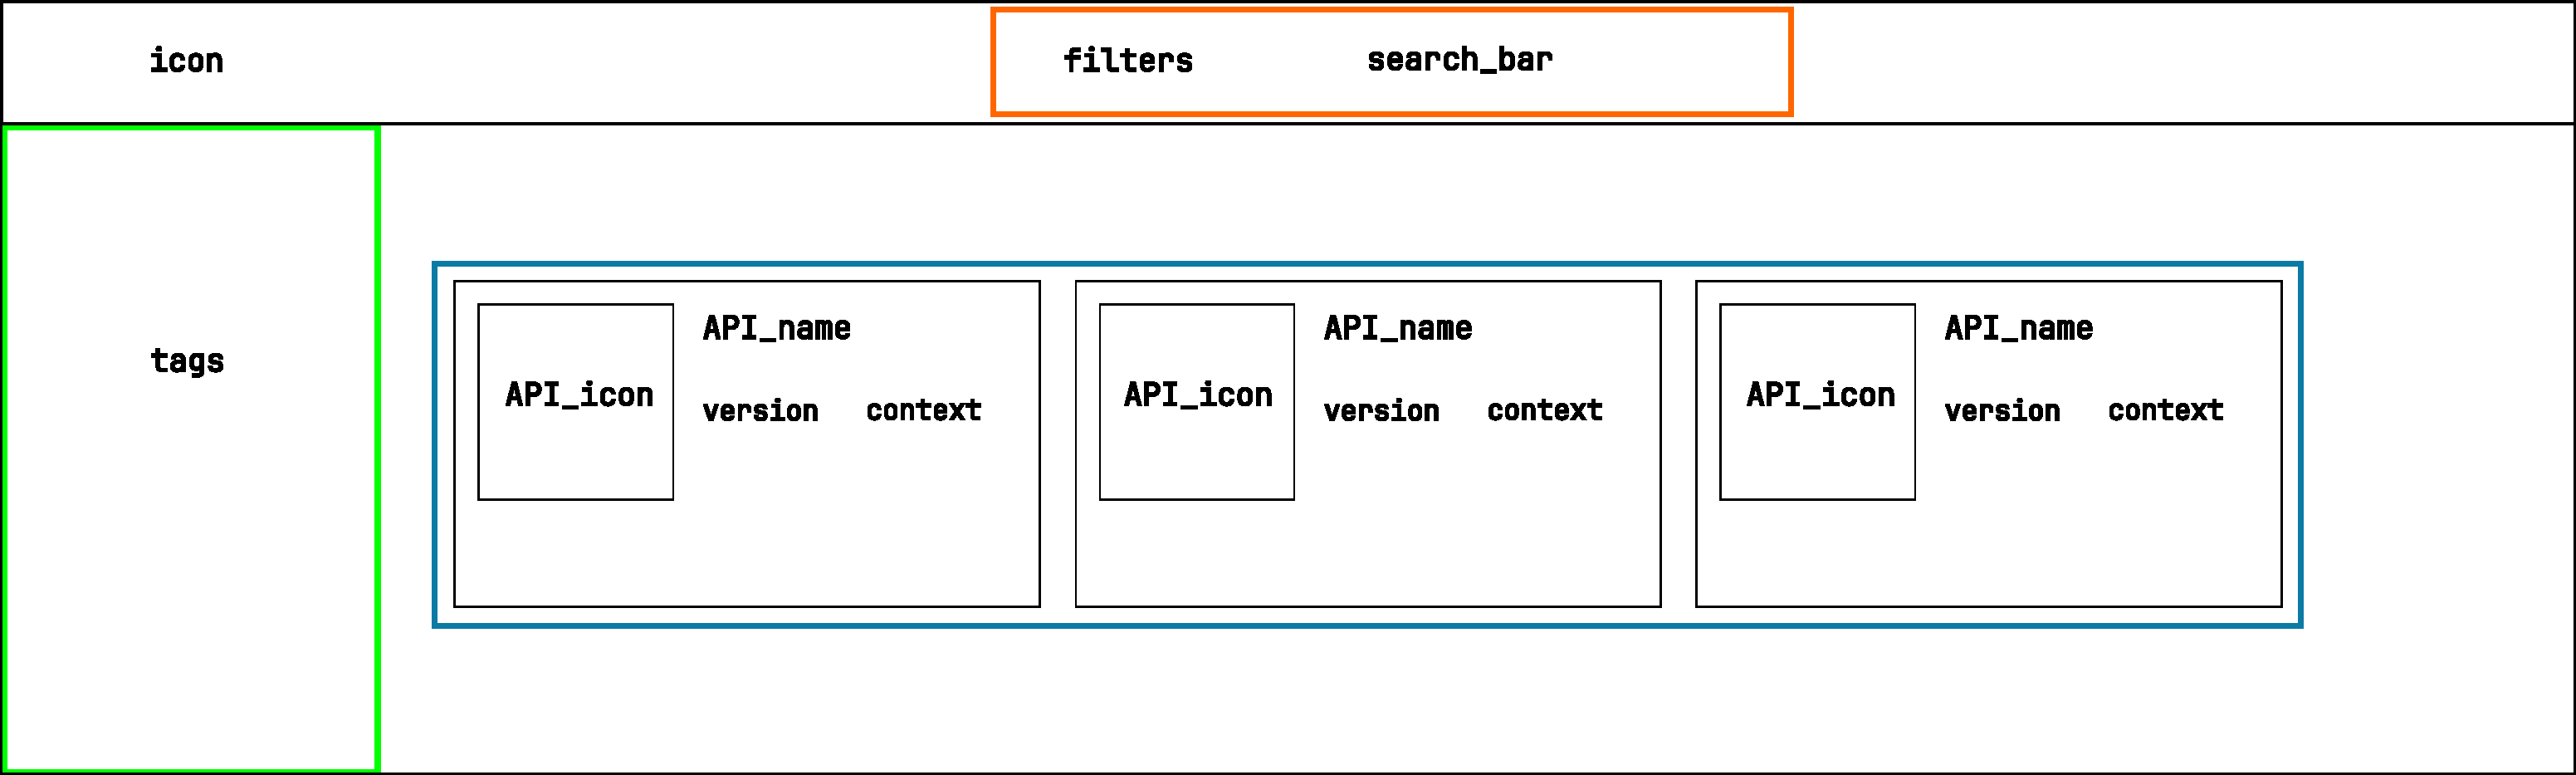
\includegraphics[width=0.95\textwidth]{img/home_mock_up.pdf}
    \caption{Mock-up de la page d'accueil}
\end{figure}


\subsection{Page de documentation}
La page de documentation détaillera la documentation de l'API utilisant la mise en page de Redoc Community Edition\footnote{Voir \href{https://redocly.com/docs/redoc}{Redoc CE} disposant d'une démonstration interactive de l'interface \href{https://redocly.github.io/redoc/}{ici}}.

\begin{figure}[H]
    \centering
    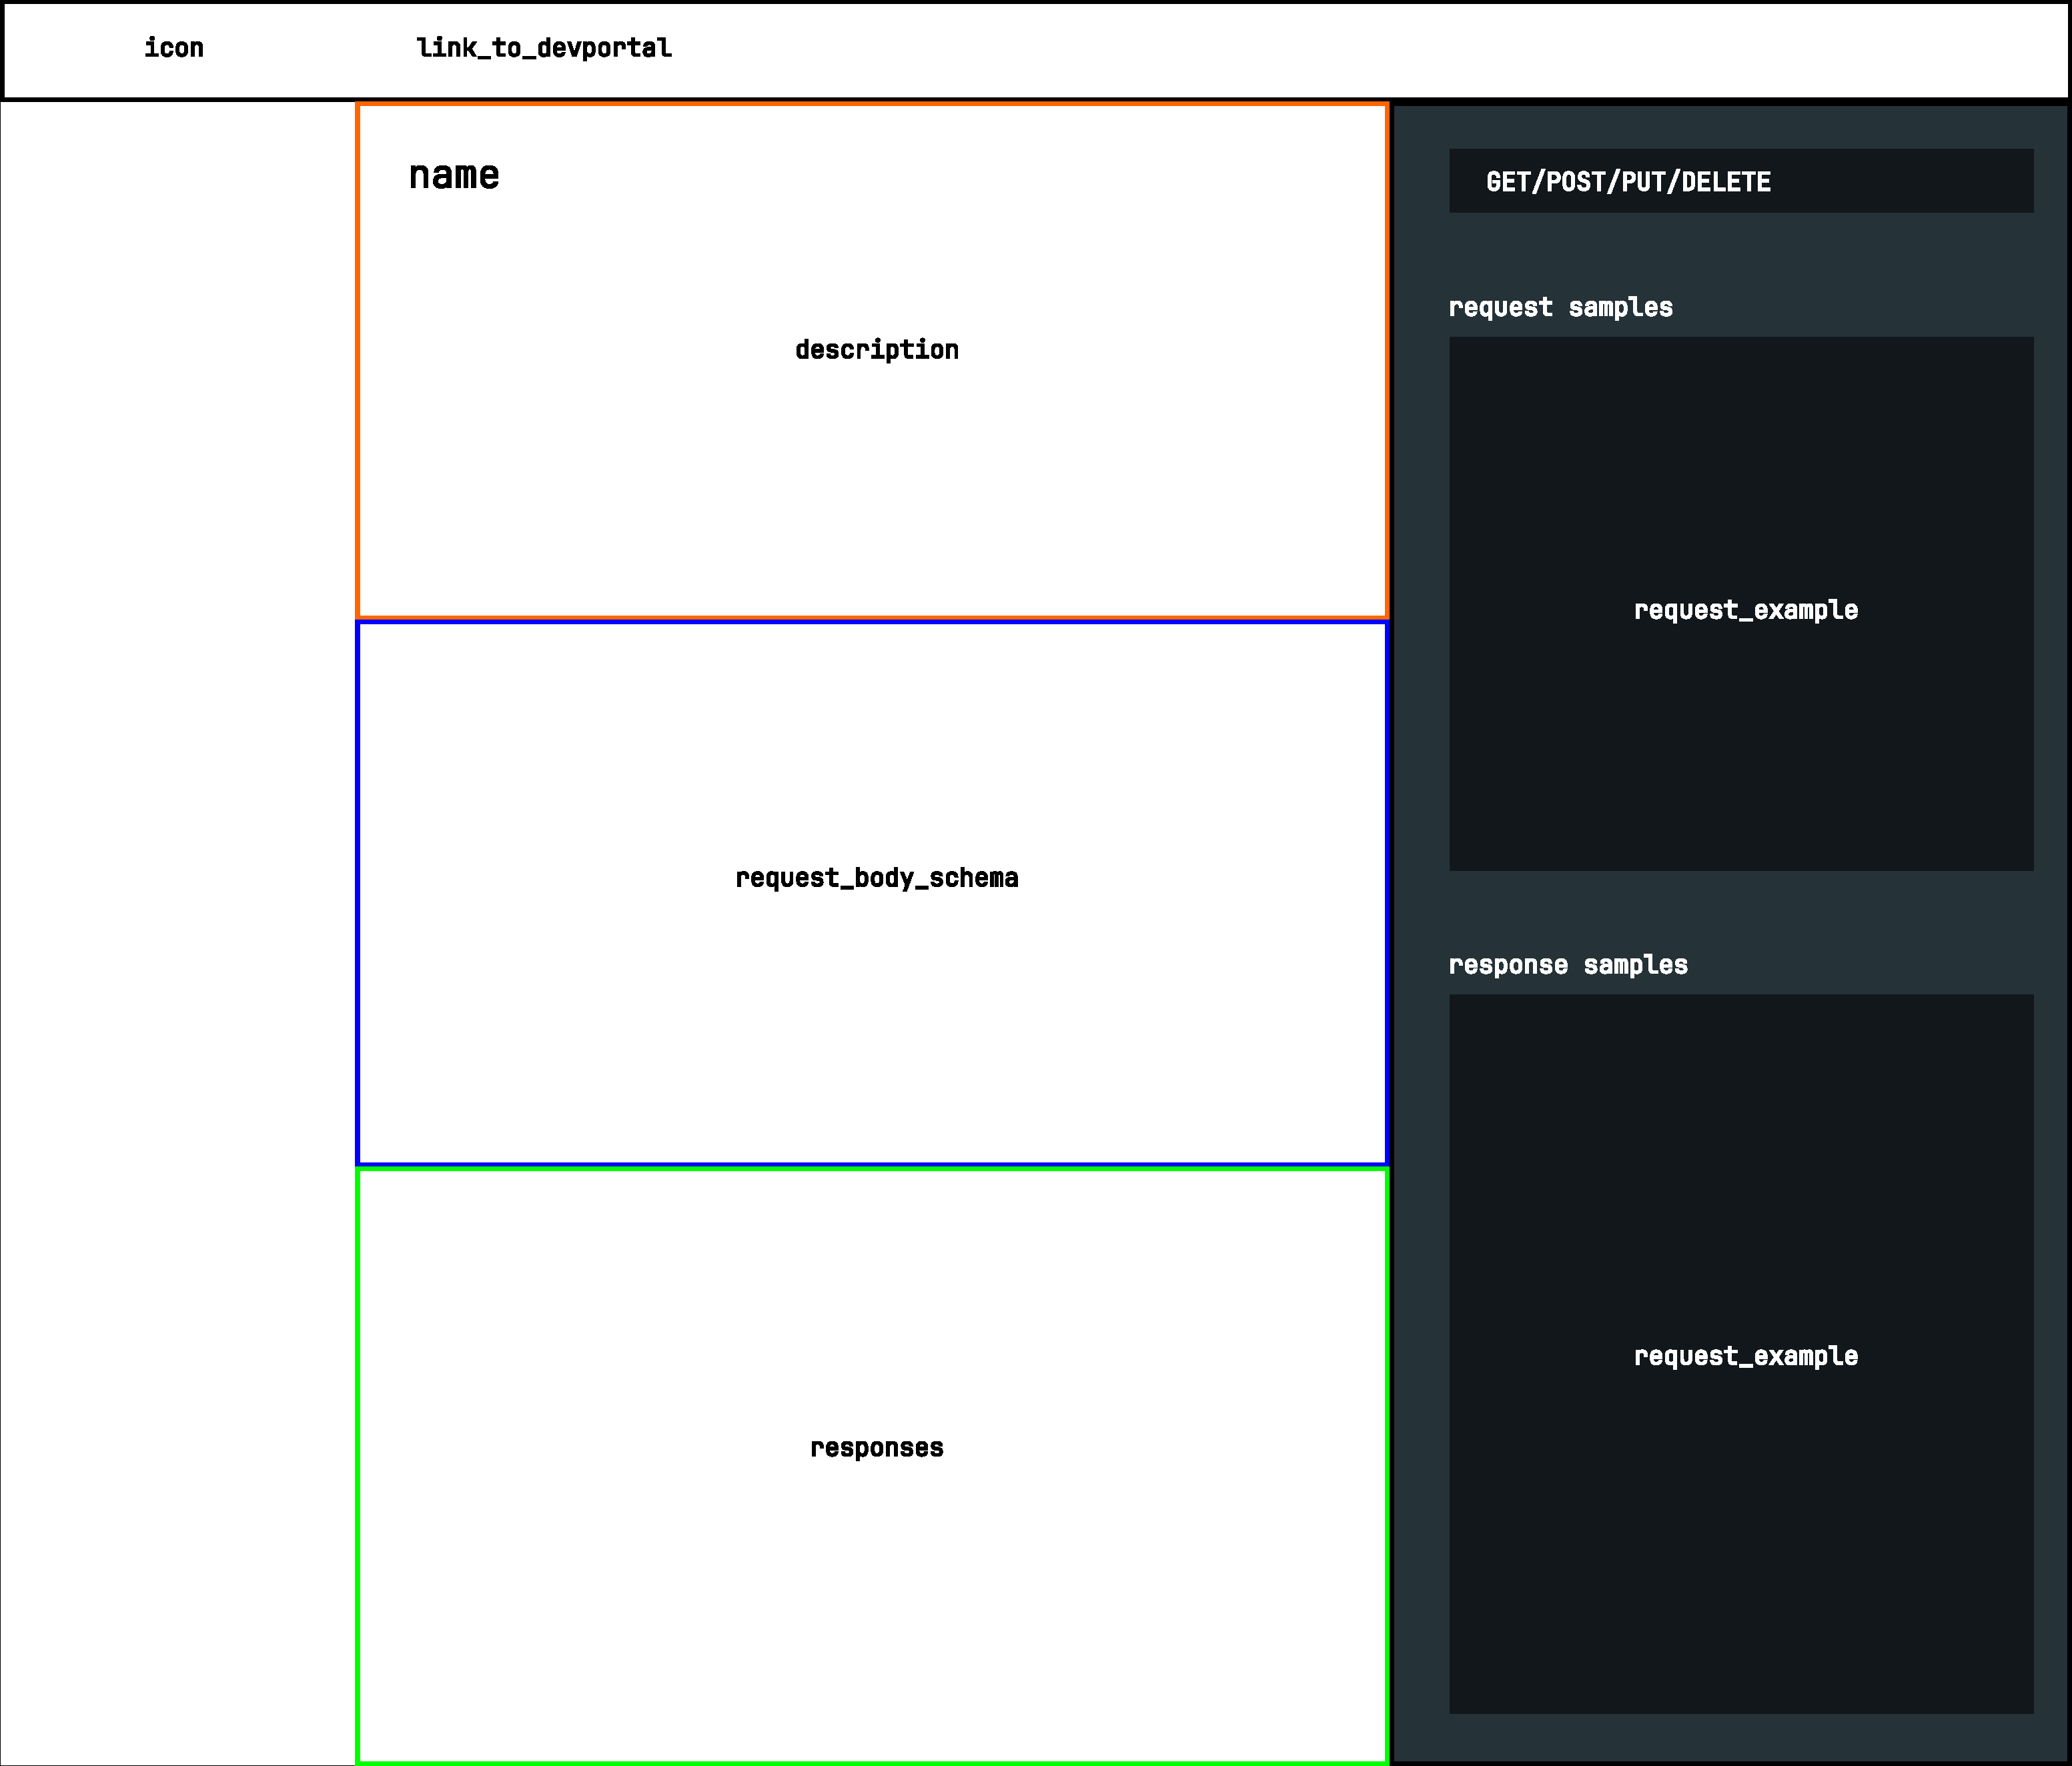
\includegraphics[width=0.95\textwidth]{img/API_mock_up.pdf}
    \caption{Mock-up de la page de documentation}
\end{figure}

%%%%%%%%%%%%%%%%%%%%%%%%%%%%%%%%%%%%%%%%%%%%%%%%%%%%%%%%%%%%%%%%%%%%%